% ============================================================================
%  Chapter 3. Methodology  (Morgan State MS format)
%
%  \input file. Parent (main_msu.tex) supplies report/12pt, double spacing,
%  Times, booktabs, graphicx, float, amsmath, natbib and .
%
%  PROVENANCE. Every reported quantity comes from results/accord/VERIFIED_FACTS.json.
%  Configuration constants (hyperparameters, pre-registered thresholds, rule
%  parameters) are cited inline to the committed source that defines them.
%  Quantities in the legacy draft chapters with no entry in VERIFIED_FACTS.json
%  are not restated. This chapter reports no outcomes; outcomes are Chapter 4.
% ============================================================================

\chapter{Methodology}
\label{ch:method}

\section{What This Chapter Specifies}
\label{sec:m-overview}

This chapter describes the pipeline that was built and, for each stage, the control designed to
separate a real finding from an artifact of the measurement. A control is informative only if the
condition under which it would fire is fixed before the number arrives, so every control below is
written as a condition, and Chapter~\ref{ch:results} reports which conditions were met.

The pipeline has four stages and an evaluation layer. Stage one extracts a cohort of admissions from
MIMIC-III and, for each, a paired nursing note and discharge summary. Stage two mines that corpus
with four rules to produce a pool of contradiction candidates. Stage three labels the pool with a
local language model. Stage four trains a neural detector on those labels and scores it against a
pharmacist-annotated gold set. Each stage inherits the previous stage's defects, which is why the
controls are given stage by stage rather than collected at the end. Two absences are deliberate:
there are no results here beyond counts registered in the project's verified-fact file with a
producing artifact, and there is no attempt to present the design as intended rather than as it
ran, because a methods chapter documenting the specification instead of the implementation is the
failure this thesis is about.

\section{Data and Cohort}
\label{sec:m-data}

\subsection{Source, access and text handling}

All clinical experiments use MIMIC-III v1.4 \citep{johnson2016mimic}, a de-identified critical-care
database from one academic medical centre. MIMIC-III is credentialed data; access came through the
standard PhysioNet route under a data use agreement, and that agreement determined how the analysis
was arranged. Four tables are used: \texttt{ADMISSIONS} for admission and discharge timestamps,
\texttt{PATIENTS} for the subject identifier used in grouping, \texttt{DIAGNOSES\_ICD} for the
ICD-9 codes defining the cohort, and \texttt{NOTEEVENTS} for the notes with their category label
and chart date.

No clinical note text appears in this thesis, in any table, figure, appendix or released artifact,
and no admission or subject identifier is printed anywhere. Note-derived intermediate files live
outside the version-controlled tree and never leave the analysis machine, and the export script
scans candidate files for note-text markers and aborts rather than filtering on a hit. Sentence
pairs were, in several runs, also sent to hosted model APIs; Section~\ref{sec:m-ethics} states why
every result obtained that way has been withdrawn from this thesis rather than reported.

MIMIC-III notes are de-identified by an automated system that replaces protected health information
with bracketed surrogate tokens \citep{neamatullah2008deid}. That is not neutral for a model
reading a fixed-length prefix, because surrogates cluster at the head of a note where name, date,
service and identifier fields sit. A model truncating a discharge summary to its first few hundred
WordPiece tokens is therefore reading an administrative header for some unknown fraction of notes,
which is a property of the data representation rather than of the modelling.

\subsection{Cohort definition}

The primary cohort is heart failure, chosen because polypharmacy is the norm in this population and
the drugs involved, among them loop diuretics and anticoagulants, have narrow therapeutic windows
and documented harm when continued inappropriately. Admissions enter if any ICD-9 code matches the
prefix \texttt{428}; two secondary cohorts were built for a transfer test, sepsis under \texttt{038}
and acute kidney injury under \texttt{584}. A prefix match on a billing code is weaker than the
physiologic criteria a clinical study would use, since it over-includes admissions where heart
failure is a comorbidity and under-includes admissions where the condition was present but uncoded.

The only further clinical filter is a positive length of stay. Applying the prefix match alone
returns 13,608 heart failure admissions; after the length-of-stay filter 13,597 remain, of which
10,143 belong to distinct subjects. The two secondary cohorts move by the same filter from 6,265 to
6,253 admissions for sepsis and from 11,422 to 11,408 for acute kidney injury, removing 12 and 14
admissions respectively against 11 for heart failure, in every case under one percent of the cohort.

\subsection{Note roles}

The clinical hypothesis is that note types carry different institutional weight. A nursing progress
note recording that a diuretic was withheld is an account of what happened at the bedside; a
discharge summary instructing that the same diuretic be continued at a stated dose is an order
governing the patient after discharge. A disagreement between the two is asymmetric, because only
one of them is the document the patient and the receiving clinician act on.

A three-role partition adding a physician or admission note was tried and dropped: physician note
types in MIMIC-III are unevenly populated across the covered period, and requiring three roles at
once intersects three sparse conditions, so no configuration reached usable coverage. Dropping the
third role is a design cost rather than a nuisance, since a two-role partition cannot separate a
nursing-to-physician disagreement, a within-stay communication failure, from a nursing-to-discharge
disagreement, a failure that reaches the patient. The adopted partition maps
\texttt{discharge summary} to the discharge role, maps \texttt{nursing} and \texttt{nursing/other}
to the nursing role, and discards every other category. It finds 13,321 of the 13,608 heart failure
admissions with a discharge summary and 10,012 with a nursing note; the intersection carrying both
roles is 9,820 admissions, the figure this thesis prints throughout.

One note per role per admission is then selected. The nursing note is the one with the latest
\texttt{CHARTTIME} strictly earlier than \texttt{DISCHTIME}, the last documented bedside state
before the patient leaves. The discharge summary is the first row under a deterministic ordering by
\texttt{CHARTDATE} with the row identifier as tie-break, since \texttt{CHARTTIME} is null for every
discharge-summary row in MIMIC-III: these notes are written retrospectively and only a
\texttt{CHARTDATE} is recorded. That ordering restores determinism, not sub-day chronology, which
the resource does not contain. Two consequences constrain later claims. Every statement that the
nursing note came first rests on the selection rule rather than on a measured comparison, and any
filter searching for documentation written between the two notes at sub-day resolution has an empty
interval to search: at that resolution the intermediate-documentation hypothesis is untestable in
this resource rather than tested and rejected. Counting at date-level resolution instead is a
coarser but answerable question, and Section~\ref{sec:m-candidates} reports it directly.

This selection returns 9,783 admissions with a selected nursing note and 9,783 with a selected
discharge summary, for 19,566 note rows across 9,783 pairs in total, 37 fewer than the 9,820
admissions carrying both roles; the shortfall is entirely nursing-side. Holding the nursing role
means holding at least one note labelled nursing; being selectable means holding one whose chart
time is recorded and falls strictly before the discharge time. An admission whose nursing notes all
carry a null chart time, or all fall at or after discharge, therefore has the role and no selectable
note, while the discharge side applies no such condition and loses nothing. That is the cohort the
mining rules of Section~\ref{sec:m-candidates} run against. Figure~\ref{fig:cohort-flow} carries the
whole path: admissions selected by billing code, filtered on length of stay, reduced to those
carrying both note roles, and reduced again to one note pair per admission; the medication mentions
extracted from those pairs and the subset carrying an action class; the candidates the four mining
rules return after the temporal prefilter; and the pairs a pharmacist annotated. The terminal box is
the non-ambiguous evaluation core and the confirmed contradictions inside it.

\begin{figure}[!t]

\centering
\caption[Cohort flow from the source database to the evaluated sets]{The path
from the source database to the evaluated sets, with the count at each stage and
the exclusions recorded as counts. Two intermediate exclusions are not drawn
because no committed file records either as a count.}
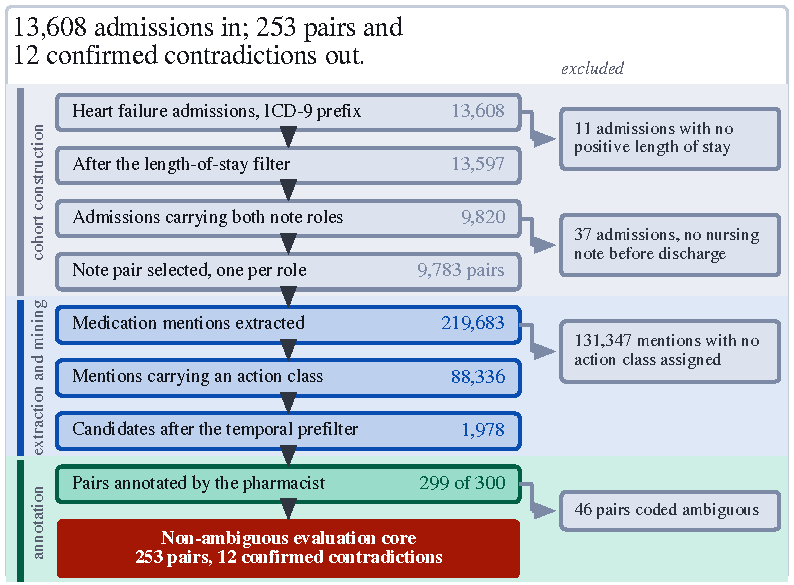
\includegraphics[width=0.88\linewidth]{figures/fig-cohort-flow.pdf}
\label{fig:cohort-flow}
\end{figure}

\subsection{Medication mention extraction and splitting}

Medication extraction is a mature task with strong published systems
\citep{uzuner2010medication,henry2020n2c2} and mature tooling
\citep{neumann2019scispacy,eyre2021medspacy}. This project used neither, after installation of both
failed against the pinned environment; the pipeline instead uses a dictionary extractor over a
general-purpose English pipeline. That is a limitation, not a considered choice.

The extractor uses four hand-written resources: heart-failure-relevant generic drug names;
abbreviation and brand-name expansions; spelling and formulation normalisations, so formulations of
one agent collapse to a single target; and regular expression alternations defining the action
classes cessation, continuation, initiation and dose modification, plus a separate negation
alternation. Matching is case-insensitive with word boundaries on both sides, applied after
expansion. Action classification operates on a window of three sentences, the previous, current and
next: the negation alternation produces a boolean over that window, the four action alternations
are applied in a fixed order and the first match determines the raw action, and negation then
rewrites the result, mapping continuation and initiation to cessation and cessation to
continuation.

Run over the 9,783 admissions the extractor returns 219,683 mentions across 9,732 unique admissions
and 70 distinct drugs, of which 88,336 receive an action classification and 131,347 do not. Fewer
than half of all mentions carry an action at all, which bounds how much of the corpus Rules 1 and 2
can ever reach, since both rules are defined entirely over the classified subset.

Three properties propagate downstream: the action is a property of the window and not of the drug
mention, so every drug named anywhere in the window gets the same label; first-match ordering makes
the classes non-exclusive in effect, since a window carrying vocabulary from two classes resolves
to whichever is tested first; and the negation rewrite is a hard flip with no scope model, where a
purpose-built context algorithm would model scope explicitly \citep{chapman2001negex}.

Two fields exist only in the rebuild: a numeric dose parser reducing a matched dose string to a
value and a canonical unit, converting within the mass family and leaving other unit families
incomparable since conversion needs drug-specific information the resource lacks, and a sentence
index and character offset on every mention, without which the defect in Section~\ref{sec:m-exemplar}
is enabled, since two mentions of the same drug in one note are otherwise indistinguishable rows.

Candidates concentrate within admissions and the patient population has repeat admissions, so a
row-level split would place candidates sharing a nursing note, a discharge summary, an admission or
a patient on both sides, since two candidates from one admission differ only in the drug at issue
while the surrounding text and documentation style are identical. Every split used here is instead
disjoint by \texttt{SUBJECT\_ID}, asserted in code rather than assumed:
\[
S_{\text{train}} \cap S_{\text{val}} = S_{\text{train}} \cap S_{\text{test}}
= S_{\text{val}} \cap S_{\text{test}} = \varnothing ,
\qquad
S_{\text{train}} \cup S_{\text{val}} \cup S_{\text{test}} = S .
\]
Patient-level grouping is the correct unit because it is the only unit guaranteeing no shared note
and no shared documentation episode. Row-level decontamination is weaker still, since a subject can
contribute one admission to the gold set and another to the weak-label pool, so the control
training pool of Section~\ref{sec:m-control-model} excludes, by assertion, every weak-label row
whose subject appears in the gold set.

\section{Candidate Generation}
\label{sec:m-candidates}

\subsection{Formulation}

True cross-note medication contradictions are rare, exhaustive human review of the cohort is
infeasible, and exhaustive machine scoring of all cross-note drug pairs is both wasteful and
statistically hostile. Candidate generation is the standard response: a cheap, high-recall,
low-precision rule set narrows the space to a pool a human or a model can examine. The rules are
not intended to be accurate, only transparent, so each candidate carries a reason, and enriching, so
the base rate inside the pool exceeds the rate outside it.

Let admission $a$ have a nursing note $N_a$ and a discharge summary $D_a$, with mention sets
$M(N_a)$ and $M(D_a)$. Each mention $m$ carries a normalised drug $\mathrm{drug}(m)$, an action
label $\mathrm{act}(m) \in \{\textsc{cess}, \textsc{cont}, \textsc{init}, \textsc{dose},
\textsc{unc}\}$, an optional numeric dose $(\mathrm{val}(m), \mathrm{unit}(m))$, a sentence
$\mathrm{sent}(m)$ and, in the rebuild only, a position $\mathrm{pos}(m)$. A candidate is a tuple
$c = (a, r, d, m_N, m_D)$, where $r$ indexes the rule, $d$ is the drug or drug pair at issue, and
$(m_N, m_D)$ is the exemplar pair, the single mention from each note presented as evidence. The
distinction this section turns on is between the trigger predicate $T_r(a,d)$, which decides
whether a candidate exists, and the exemplar selector $E_r(a,d)$, which decides what evidence
accompanies it. A correct implementation requires that $T_r$ holding implies $\mathrm{act}(m_N)$
and $\mathrm{act}(m_D)$ are the two actions that made it hold.

\subsection{The four rules}

Rule 1 fires when the same drug appears in both notes and the action sets disagree in a specific
direction. With $A_N = \{\mathrm{act}(m) : m \in M(N_a),\ \mathrm{drug}(m) = d\}$ and $A_D$ defined
analogously,
\[
T_1(a,d) =
(\textsc{cont} \in A_N \wedge \textsc{cess} \in A_D)
\;\vee\;
(\textsc{cess} \in A_N \wedge \textsc{cont} \in A_D).
\]
This is the canonical case: the nursing note records the drug as held and the discharge summary
orders it continued, or the reverse. The existential quantifier means the rule fires if some
mention on each side carries the required action, correct for a high-recall trigger and exactly
what makes exemplar selection non-trivial.

Rule 2 relaxes drug identity to pharmacologic class, so two different agents in one class, one
continued and one ceased across the notes, can be flagged as a substitution documented on one side
only. It uses a hand-written class dictionary covering the major heart-failure classes, plus a
guard that the drug sets on the two sides are not identical, which would return the candidate to
Rule 1. The dictionary is small relative to the pharmacologic space, is not derived from a standard
terminology such as ATC or RxNorm, encodes one author's judgement at its boundaries, and has no
mechanism for cross-class interactions.

Rule 3 fires when the same drug carries a parseable numeric dose in both notes, the doses reduce to
the same canonical unit, and they differ by more than a fixed fraction of the larger value:
\[
T_3(a,d) = \exists\,(m_N, m_D):\
\mathrm{unit}(m_N) = \mathrm{unit}(m_D)\ \wedge\
\frac{\max - \min}{\max} > \tau ,
\]
with $\tau$ fixed at $0.20$ in the mining implementation. The threshold is a judgement call
with no empirical derivation, it is not tuned, and it is not clinically grounded, since a given
proportional change in a statin dose and the same change in a warfarin dose are not comparable
events. Its exemplar selection is correct by construction, because the exemplar is the pair
achieving the largest proportional difference.

Rule 4 fires when a drug receives a cessation action in the nursing note and is absent from every
extracted mention in the discharge summary, classified or not:
\[
T_4(a,d) =
\bigl(\exists\, m \in M(N_a):\ \mathrm{drug}(m) = d \wedge \mathrm{act}(m) = \textsc{cess}\bigr)
\;\wedge\;
d \notin \{\mathrm{drug}(m) : m \in M(D_a)\}.
\]
This is the clinically most interesting rule and the weakest in evidence, since absence is not a
decision: a drug held at the bedside and never mentioned again may have been deliberately
discontinued and correctly omitted, or dropped by oversight, and the rule cannot tell them apart. It
also produces a structurally different input, since there is no discharge sentence to show and the
discharge side is a literal marker, so any difference in labeller or model behaviour on Rule 4 has
at least two explanations, clinical reasoning and a formatting response to a degenerate input,
which the design cannot separate.

Rules 3 and 4 exist only in the rebuild, since the reference extractor never parsed dose strings or
recorded positional information; comparison between rebuild and reference behaviour is therefore
restricted to Rules 1 and 2, which is what defines the defect-free stratum used in
Section~\ref{sec:m-control-rq1}.

Applied to the classified mentions, the four rules return a raw pool of 1,980 candidates before any
temporal check, split 886 from Rule 1, 203 from Rule 2, 521 from Rule 3 and 370 from Rule 4,
covering 1,205 distinct admissions. A temporal prefilter requiring a resolvable ordering between the
two notes drops the pool to 1,978 candidates, split 886, 202, 520 and 370, out of 1,068 admissions
carrying a usable date window and 643 carrying an intermediate note between the two selected notes.
Every candidate count elsewhere in this thesis is the post-prefilter figure, 1,978, unless stated
otherwise.

\subsection{Exemplar selection, and the defect in it}
\label{sec:m-exemplar}

The reference mining code for Rules 1 and 2 selects the exemplar by positional index into the
drug's mention group, taking the first row on each side, with nothing constraining those rows to
carry the actions that made the trigger true. If a discharge summary mentions a drug several times,
mostly continuation with one later cessation, while the nursing note has a single continuation
mention, the trigger fires on the continuation-cessation branch and the candidate is real by the
rule's own definition, but the positional selector returns a continuation row on the discharge side,
so the exemplar presented as a contradiction consists of two sentences in which the notes agree.

This is a methods matter rather than an incidental bug: the pharmacist annotated the exemplar pair,
the weak labeller read it, and the detector was trained on it, so wherever the selector failed, all
three reasoned about evidence that did not contain the conflict which caused the candidate to exist.
The defect was invisible because of an upstream schema decision rather than a typo: with no sentence
index and no character offset, two mentions of one drug in one note are indistinguishable rows, so
positional selection is not obviously different from any other choice, and there was no
representation in which the mention carrying the conflict could be expressed. This is configuration
and data-dependency debt in the sense of \citet{sculley2015debt}, a defect made unreachable by the
absence of the field that would have exposed it.

The rebuild selects, on each side independently, among only those mentions whose own action equals
the action required by that candidate's conflict branch:
\[
E_r^{\text{new}}(a,d) = \Bigl(\arg\min_{m \in C_N} \delta(m),\;
\arg\min_{m \in C_D} \delta(m)\Bigr),
\quad
C_X = \{m : \mathrm{drug}(m) = d,\ \mathrm{act}(m) = \rho_X\},
\]
where $(\rho_N, \rho_D)$ is the action pair required by the branch that fired and $\delta(m)$ is
the character distance from $m$ to the nearest dose-bearing mention in the same note. The tie-break
is a heuristic with a stated rationale and no validation: a mention adjacent to a concrete dose is
more likely to be a substantive instruction than a passing reference in an allergy or problem list,
and with no dose-bearing mention it falls back to the earliest qualifying sentence for determinism.
Because it chooses among mentions that already qualify it cannot reintroduce the original defect,
and whether it changes a clinical judgement was not measured.

\section{Weak Supervision}
\label{sec:m-weak}

\subsection{Labeller, pool and prompt protocol}

Training a supervised detector on a few hundred annotations containing a handful of positives is
not viable, so this project uses weak supervision: obtain approximate labels cheaply, accept that
they are noisy, and rely on the model to average over the noise \citep{ratner2017snorkel}. Since
2023 the dominant cheap labeller has been an instruction-tuned language model, on the strength of
results showing such models matching or exceeding crowd annotators on several classification tasks
\citep{gilardi2023chatgpt}.

The production labeller is Llama 3 8B \citep{grattafiori2024llama3}, run locally and presented with
each candidate's exemplar sentence pair and the identifier of the rule that generated it, asked for
a binary judgement plus a confidence value. The prompt is a fixed template with no demonstrations
and no chain-of-thought elicitation, and it names a conflict type before asking whether a conflict
is present. The labelled pool is the candidate pool minus the pairs put to the pharmacist, disjoint
at the row level by construction; Section~\ref{sec:m-data} explains why that was insufficient. The
weak-labelled candidate pool from this calibration join holds 1,679 rows before subject-disjoint
exclusion; removing the 291 rows whose subject also appears in an evaluation split leaves 1,388,
split into the 1,183-row training pool reported in Table~\ref{tab:m-strata} and used to fit the
detector, and a 205-row validation pool used only to monitor the training loss.

For the replication in Section~\ref{sec:m-control-rq2} the evaluation baseline's prompt was
recovered verbatim from the committed prompt table rather than rewritten, and reused unchanged
across models. It is not the deployed weak labeller's prompt, which the table does not contain, so
the replication reproduces the baseline configuration rather than the configuration that produced
the training labels; the deployed run and the same model's baseline-prompt replication differ by
$165$ positive labels across the full pool, a lower bound on the rows they disagree on (Section~\ref{sec:res-rq2}). Decoding is greedy at temperature zero
for the local models, so a model's label for a row is deterministic within a model. Generations that
do not parse are recorded in their own category and never defaulted to a class, which would otherwise
inflate a positive rate mechanically and silently.

\subsection{How \texttt{weak\_confidence} was derived}

The labelling stage emits a \texttt{weak\_confidence} field alongside each label. Across the
training pool and the audited rows it takes exactly two distinct values, one for each label class,
in a one-to-one mapping, so it is a deterministic function of the label and carries no information
about the labeller's uncertainty on any individual example.

The field was used in two places, both converting a label into a training-time intervention. As a
filter, the training code discards rows whose confidence falls below a threshold lying beneath the
field's minimum value, so the filter removes nothing while reading, in the code and in every
description of the pipeline, as a quality-control step. As a loss weight, the same field is
multiplied into the per-example loss, making it a label-conditioned reweighting rather than a
confidence weighting, in the direction that further downweights the already-dominant class. A
confidence value emitted by a language model alongside a label is not a calibrated probability and
should not be treated as one without measurement \citep{guo2017calibration,zhao2021calibrate}.

Weak labels are used only as training supervision here, never as ground truth, so any metric
computed against them measures agreement with the labeller rather than clinical correctness.
Validation of an automated annotation procedure against human labels on the same items is a
requirement rather than an option \citep{pangakis2023validation}, and the gold set of
Section~\ref{sec:m-gold} supplies those items.

\section{The Detector}
\label{sec:m-detector}

\subsection{Backbone, and what the running code contained}

The encoder is BioMedBERT (released as PubMedBERT) \citep{gu2021biomedbert}, selected over ClinicalBERT
\citep{alsentzer2019clinicalbert} on published benchmark performance, adapted with low-rank
adapters on the attention projections \citep{hu2022lora}. Each candidate's nursing and discharge
sentences are encoded, each truncated to a fixed prefix from the head of the sequence, which is
where Section~\ref{sec:m-data}'s observation about the de-identification header applies. The system
was specified as that backbone plus four purpose-built components: a cross-note difference encoder,
an asymmetric conditioning module, a pharmacological prior conditioning module, and a
guideline-grounded harm estimator, with three claimed contributions attached to them. What follows
describes the code that produced the results rather than the specification, per the correction
recorded as C4, one of the entries named but not reproduced in Appendix~\ref{app:corrections}.

The pharmacological prior module was deleted in the second version and replaced by a function
returning a fixed-length vector of zeros with two positions overwritten, one a danger multiplier
and one a normalised rule identifier. It has zero learned parameters, and the running code contains
no drug class table, no interaction table and no contraindication list.

The guideline-grounded harm estimator has no guideline corpus: its guideline bank is a single
randomly initialised parameter matrix cross-attended from one query, with no document collection,
index, retrieval step or text of any kind. More consequentially, the harm head and the explanation
head receive no loss term, since the objective is a weighted sum of only the contradiction loss and
the rule-type loss, so both heads are randomly initialised modules whose outputs are computed,
recorded and reported while their weights never move; the severity-ranking question was therefore
not tested, and any correlation between that head's output and a human danger rating measures an
untrained module rather than severity ranking.

The auxiliary rule-type head predicts the rule identifier that the prior-feature constructor writes
into the model's input, one linear layer apart in the same forward pass, so the task is a copy
operation. Auxiliary-label leakage of this shape belongs to a documented family
\citep{poliak2018hypothesis,gururangan2018artifacts,mccoy2019hans,geirhos2020shortcut}: an auxiliary
head whose target is derivable from its own input features is not an auxiliary task, and the
cheapest test is out-of-domain transfer rather than held-out accuracy \citep{zech2018generalization}.

The asymmetric conditioning module carries a two-element authority parameter initialised at the
pair of values later reported as discovered, applied to a cross-attention branch that is
immediately layer-normalised. Layer normalisation is invariant to a per-branch scalar rescaling of
its input up to the effect on its own affine parameters, so the normalisation removes most of what
the parameter does and the gradient reaching it is correspondingly small. The diagnostic that
follows is stated as a rule and applied in Chapter~\ref{ch:results}: for any parameter reported as
learned, publish its relative displacement from initialisation and a gradient-norm trace.

\subsection{Pretraining, and an untrained configuration}

Before supervised training the model was to be pretrained with a cross-note coherence objective,
discriminating genuine note pairs from mismatched ones. One configuration has a surviving run
record, with a frozen backbone; a wider configuration, meant to test whether trainable capacity
rather than architecture was the constraint, was never trained. The Stage 0 training script freezes
the backbone unconditionally with no code path that unfreezes any encoder layer, and the parameter
total attributed to the wider configuration is reconstructible only by counting a pooler module
that a forward and backward pass confirmed carries gradient flags and no gradient
(Appendix~\ref{app:corrections}, C54).

No claim of the form ``X was never trained'' may rest on the absence of a checkpoint, since a
checkpoint for the wider configuration does exist on a drive mount an earlier search did not reach
(Appendix~\ref{app:corrections}, R6); the claim here rests on the code path and the gradient check
alone.

\subsection{The defect-free control model}
\label{sec:m-control-model}

Because the detector carries documented defects, a null measured on it alone cannot be attributed
to the task. A second model was built as a control rather than a competitor, and it is deliberately
boring. The nursing and discharge sentences are concatenated with separator tokens, passed through
BioMedBERT, and the raw first-token hidden state feeds one linear layer producing one logit under a
binary cross-entropy objective. There is no rule feature, no authority parameter, no auxiliary
head, no harm head and no confidence reweighting, since any of those would reintroduce a defect the
control exists to rule out.

The training protocol is fixed and reported in full. The train and validation split is drawn by
subject with a dedicated split seed held fixed across runs, so variation between runs reflects
model stochasticity and not different training data, and the seed setter is called inside each
run's own process, one process per seed, so no session state carries across runs. Optimisation uses
AdamW at learning rate $2\times 10^{-5}$ with weight decay $0.01$, batch size 16, three epochs and a
maximum sequence length of 160 tokens, all fixed rather than swept.

Two floor baselines are trained on the identical pool and split so the comparison is like for like:
a majority-class predictor assigning every gold row a constant score equal to the training-pool
positive rate, and a TF-IDF representation with at most $5{,}000$ features feeding logistic
regression. The constant score yields an AUROC of exactly $0.5$ by construction, making it the
correct reference point for reading any AUROC near chance.

\section{The Gold Standard}
\label{sec:m-gold}

\subsection{Sampling and annotation protocol}

A stratified sample was drawn from the candidate pool, allocated across the four rules in
proportion to each rule's share of the pool (886, 202, 520 and 370 candidates for Rules 1 through
4), rounded to whole pairs and not oversampled toward any rule. The frame draws 134 pairs from Rule
1, 31 from Rule 2, 79 from Rule 3 and 56 from Rule 4, for 300 pairs total, the same sampling
fraction in every stratum to within rounding, and was fixed before annotation began. Proportional
allocation has a consequence Chapter~\ref{ch:results} relies on: under it, the gold sample's base
rate is an unbiased estimate of the pool's base rate, the denominator the over-calling ratios in
that chapter divide against. The returned annotation set has $n = 299$ pairs, one fewer than the
frame; the per-rule breakdown, 134, 31, 79 and 55, shows the missing row belongs to Rule 4, since
Rules 1 through 3 returned every sampled pair and Rule 4 returned one fewer than it was sent.

A single board-certified pharmacist annotated the sampled pairs, recording for each a three-way
label, contradiction, not a contradiction, or ambiguous; a free-text justification; a confidence
rating; and, for contradictions, an ordinal danger rating. The annotator saw the exemplar sentence
pair and the rule that generated the candidate, which is the same evidence the weak labeller and
the detector saw. Annotation ran in two passes separated by a two-week washout. The two-pass design
controls for within-session drift and fatigue, and that is all it controls for; it does not
establish inter-rater reliability, because there is one rater.

\subsection{The ambiguity category}

A pair was coded ambiguous when the presented evidence did not permit adjudication, rather than
being forced into a binary that would have converted an evidential limitation into a label
indistinguishable from a genuine negative. The category has a cost in the evaluation layer, handled
by reporting both readings rather than choosing one: ambiguous pairs are retained as negatives in
the primary stratum and excluded in the power calculation the project originally referenced, which
is why Section~\ref{sec:m-stats} reports the minimum detectable effect under both denominators, and
no result here is reported under only one treatment of the ambiguous rows.

\subsection{What this design can and cannot establish}

A reliability claim previously attached to this gold set is retracted here rather than in a
footnote, because the retraction concerns the instrument. The project reported a Cohen's $\kappa$ of
$1.000$ between two independent pharmacist judgement instruments, which were in fact the binary
contradiction label and the ordinal danger rating: a pair that is not a contradiction has no danger
by definition, so the agreement between a positive label and a positive danger rating is an identity
guaranteed by construction \citep{cohen1960kappa} and measures nothing about annotator reliability.

The honest statement is that this study has one annotator, a two-pass protocol with a washout, and
no established inter-rater reliability; a second annotator would be the highest-value single
addition to the work, and its absence is a first-order limitation on every conclusion resting on the
gold labels.

Intra-rater agreement is not a fallback here. The two-pass protocol reduced within-session drift and
fatigue in a single rater; it did not produce two comparable sets of judgements, since the
annotation file stores one final label per pair and the second pass overwrote the first rather than
being retained beside it. No artifact in this project keeps the pass-one and pass-two labels
separately, so a figure computed after the fact would have to be re-annotated from scratch to exist
at all. The reliability of the gold standard is therefore not a missing number the project failed to
report but one the retained record cannot produce, and every clinical result in this thesis rests on
a single-rater instrument with no inter-rater or intra-rater agreement statistic attached to it.

\begin{table}[H]
\caption[Evaluation strata and their sizes]{Evaluation strata, their sizes, and their positive counts.}
\label{tab:m-strata}
\centering
\small
\begin{tabular}{lrrl}
\toprule
\textbf{Stratum} & \textbf{$n$} & \textbf{Positives} & \textbf{Defined by} \\
\midrule
Gold, all annotated pairs & 299 & 12 & Ambiguous rows retained as negatives \\
Gold, defect-free subset  & 134 & 6  & Rules 3 and 4 only \\
Decontaminated evaluation & 253 & 12 & Ambiguous rows excluded \\
Weak-label training pool  & 1,183 & \multicolumn{2}{l}{Positive rate 0.8521} \\
\bottomrule
\end{tabular}
\apanote{The defect-free subset is fixed by rule membership before any score is computed. The training pool's positive rate is the weak labeller's marginal on the rows surviving subject-level exclusion, and it is the reference against which any agreement figure on weak labels must be read.}
\end{table}

\section{The Controls}
\label{sec:m-controls}

Each subsection states one control as a condition: what would have to be true for the corresponding
reading to survive. Every condition is written before any number in Chapter~\ref{ch:results} is
available to the reader. None of these controls is novel, and none is claimed as a contribution.

\subsection{RQ1: is the pool's precision an estimate or an upper bound?}
\label{sec:m-control-rq1}

\textbf{Condition.} If the exemplar selector agrees with its own trigger on substantially every
action-conflict candidate, the pharmacist judged the evidence that caused the candidate to exist,
and the measured precision estimates the pool's precision. If it does not agree, the measured
precision is an upper bound on the validity of the annotation exercise, and the direction of the
bias is not determinable from the data collected.

The audit instruments both selectors and records, for every action-conflict candidate, whether the
positional exemplar's action pair matched the pair required by the branch that fired, and whether
the corrected selector changed the chosen rows. Two quantities follow, an agreement rate and a
change rate, and they are not the same quantity: a candidate can change exemplar on one side while
the old exemplar happened to be correct on the other. The second half of the control is structural
rather than measured. Rules 3 and 4 have no positional selector, so the gold pairs drawn from them
form a defect-free stratum fixed before any model score exists, and every detection metric in
Chapter~\ref{ch:results} is reported on that stratum as well as on the full set. If the two strata
disagree, the exemplar defect is doing work; if they agree, it is not.

\subsection{RQ2: is the labeller's error noise or prior?}
\label{sec:m-control-rq2}

\textbf{Condition.} If a weak labeller's error were noise, its marginal would approximate the true
base rate and its mistakes would spread across classes. If its marginal sits far above the base
rate, the error is a prior shift, and no downstream aggregation removes a shifted marginal:
aggregation frameworks assume noise that is conditionally independent across sources given the true
label and rest on having multiple sources whose errors are not aligned \citep{ratner2017snorkel}.
One source with a systematic prior shift is outside that regime.

Three controls bear on this. First, ordering: the base rate must be estimated on a small
human-labelled sample before any weak labels are generated; this project produced the pharmacist
annotations after the weak labels, inverting the only ordering in which the mismatch would have
been actionable, reported here as a methods failure rather than repaired retrospectively.

Second, replication across labellers: if over-calling is a property of one model it will not
survive a change of model, but it will if it is a property of the task presentation. The
replication reruns the recovered baseline prompt unchanged over the full pool with three local
instruction-tuned models, \texttt{llama3:8b}, \texttt{granite3.3:8b} and \texttt{qwen3:8b}, served
through Ollama at temperature zero, with unparseable generations kept in their own category. Third,
a domain control: if the magnitude of over-calling generalises, a comparable labelling task on
public non-clinical text will show a comparable ratio, and if only the mechanism generalises the
ratio will be materially smaller while the direction persists, which governs what may be claimed.

\subsection{The marginal feasibility gate}
\label{sec:m-feasgate}

A thresholded labeller's flag count and the gold standard's confirmed-positive count fix, before any
score is compared, the largest attainable agreement and the smallest attainable one-sided
hypergeometric $p$ that marginal permits: placing every confirmed case inside the flagged set gives
the best table that marginal could produce. A labeller whose floor sits above the read-at threshold
could not have rejected the null however it behaved. The bound covers a hard, thresholded decision
only; a scored labeller can sweep its threshold and rank well regardless of flag rate, so this says
nothing about a ranking metric. Applied to every hard-label marginal this thesis prints, it was added
after the hosted results were withdrawn, unlike the controls above, specified before any result was
seen. The ceiling is the prevalence-and-bias problem of \citet{feinstein1990paradoxes} and
\citet{cicchetti1990resolving}, corrected by \citet{byrt1993pabak}; no novelty claim attaches to the
floor.

\subsection{RQ3: do the architectural components contribute what they are credited with?}
\label{sec:m-control-rq3}

\textbf{Condition.} A component credited with exploiting a semantic property must beat an arbitrary
substitute that carries no such property. If the arbitrary substitute matches or exceeds the
semantic feature, the credited mechanism is not the operative one, and the control has fired
positively rather than by absence of evidence. This is the control-task logic developed in the
probing literature by \citet{hewitt2019control}, applied here rather than proposed.

The arbitrary-substitute control operates on a second system in this project that conditions a
shared additive attention bias on document provenance. Seven arms were trained at three seeds each,
and three further arms at a single seed, on masked language modelling over packed multi-document
bundles, with segment order shuffled so role is decorrelated from position within the bundle: no
bias; a T5-style relative position bias; a misaligned block bias; an ALiBi-style distance bias; true
role labels; an arbitrary segment ordinal carrying no provenance meaning; and a fixed hard block
mask, the encoder analogue, under masked language modelling, of the intra-document mask
\citet{zhao2024seqcomposition} apply during causal decoder pretraining, the same mask construct but
a different training objective, disclosed here rather than treated as a reproduction. Two
comparisons are fixed in advance: true role labels against a randomised relabelling drawn from the
same alphabet, the control task in the sense of \citet{hewitt2019control}, and true role labels
against an arbitrary positional ordinal, a competing hypothesis rather than a control. The
misaligned block arm is a second control, holding the number of blocks fixed while destroying their
alignment with document boundaries, closing the reading that any coarse blocking of the attention
matrix would do.

One control, a single global derangement applying one fixed permutation to every bundle, is
deliberately not used and must not be confused with the randomised relabelling reported in
Chapter~\ref{ch:results}: since the bias table is a free matrix over role pairs, the model would
simply learn the permuted table and the loss surface is isomorphic, fixing the result at the
uncorrupted value by construction. It was implemented, recognised as powerless, and guarded against
in code, because a control that cannot fail is worse than no control.

A third control, the anisotropy control, addresses the representation rather than the mechanism.
The pretraining collapse was originally explained by clinical homogeneity, the claim that notes
within an institution are too similar for a coherence objective to separate genuine from mismatched
pairs, though nothing in the pipeline had measured note similarity. The control instead tests
whether the collapse follows from representational geometry in the encoder, passing deliberately
unrelated non-clinical sentences through the identical frozen extraction path and comparing mean
pairwise cosine similarity against matched and mismatched clinical pairs; text this similar to
itself under the same extraction weakens the homogeneity explanation without asserting the two
conditions are statistically identical, and Chapter~\ref{ch:results} reports a Welch test that
rejects exact equality.

\subsection{The degeneracy precondition}

\textbf{Condition.} Demographic parity compares the predicted-positive rate across groups, so a
classifier that predicts one class for nearly every input has the same predicted-positive rate in
every group by construction and cannot exhibit a parity disparity, whatever the underlying data. An
audit that reports no disparity on such a classifier is therefore reporting its own operating point,
not a property of the model or of the data it was run against. This is the degeneracy precondition:
a check on the validity of a parity-style audit over a binary classifier, checkable before the audit
runs. It is a precondition, not a general result about fairness metrics, and beyond what the rest of
this chapter already reports it establishes nothing about this thesis's contradiction detector.

The precondition is enforced by two mechanisms, run in order and both before the audit produces any
substantive measurement. First, a pre-registered non-degeneracy bar: the reference classifier must
clear a minimum AUROC of $0.65$, a predicted-positive rate strictly inside the interval $0.05$ to
$0.50$, and a precision lift over the base rate of at least $1.5$, all on the validation split and
all asserted in code before the sweep begins; if any of them fails, the driver exits and the sweep
does not run. Second, a planted-gap positive control, which runs immediately afterwards and checks
that the audit can detect a disparity known to be present: a known logit shift is injected into one
group's scores on the full population with no selection filtering, and the audit code must recover
it, the bootstrap interval on the demographic parity gap must exclude zero and the four-fifths ratio
must fall below its threshold with an interval upper bound below one. If the audit cannot recover a
gap placed there deliberately, every downstream number is void, and the experiment driver aborts
rather than reporting them. The precondition also applies retrospectively to an earlier audit in
this project and fails there, which is why no subgroup harm is demonstrated or claimed anywhere in
this thesis.

\subsection{RQ4: is the detector's null real?}

\textbf{Condition.} A null result is evidence only if the instrument that produced it can be shown
to resolve an effect of comparable size where one is known to exist, and only if the evaluation had
enough power to see an effect at all. Two local checks answer this together: the minimum detectable
effect for the evaluation's own sample size (Section~\ref{sec:m-mde}), and a positive control that
runs the same pretraining-effect instrument on a task where the effect is known to be present, its
outcome bound in advance to a written decision rule.

The proxy under test is whether a difference in self-supervised pretraining, measured as a loss
gap, predicts a difference in downstream discrimination. On the clinical side the comparison runs
on a task built for this control rather than on the contradiction detector: in-hospital mortality
predicted from a bundle of a patient's first 48 hours of notes, evaluated on $6{,}776$ held-out
admissions holding $570$ positives, a different task and cohort from the $253$-pair
contradiction evaluation. The comparison there is a from-scratch encoder against a
domain-pretrained encoder under a matched fine-tuning protocol at three seeds each. The two arms do
not share a seed set, so the comparison is unpaired and no per-seed difference is meaningful, and
one from-scratch run carries no recorded split lineage against the other five, so
Chapter~\ref{ch:results} reports the three-seed gap as primary and the two-seed gap over the
lineage-pinned runs alone beside it. On the public side the same comparison runs on AG News across
four arms, a pretrained BERT encoder against three from-scratch encoders at three smaller parameter
scales, with exact parameter counts given in Chapter~\ref{ch:results}.

One threat has to be answered before the public comparison can serve as a control: in the initial
sweep every arm trained for the same short budget with no per-arm tuning, so a gap between
pretrained and from-scratch arms could measure training budget rather than pretraining. The
convergence sweep instead gives every arm four budgets, each with its own complete schedule,
reported at the final epoch rather than by validation-based checkpoint selection, at three seeds per
cell, for $48$ runs and $555$ minutes of compute. The decision rule in Table~\ref{tab:m-prereg} was
committed to the project repository at commit \texttt{b048829}, before the sweep started, and
applied by the analysis notebook without being edited after the first result landed.

\begin{table}[H]
\caption[Pre-registered decision rule for the control]{Pre-registered decision rule for the pretraining positive control, committed before the
sweep was run.}
\label{tab:m-prereg}
\centering
\small
\begin{tabular}{p{0.14\linewidth}p{0.38\linewidth}p{0.40\linewidth}}
\toprule
\textbf{Outcome} & \textbf{Condition at the longest budget} & \textbf{Consequence} \\
\midrule
A & Gap of at least $3.0$ accuracy points between the largest from-scratch arm and the pretrained
    arm, and the two arms' one-standard-deviation bands do not overlap
  & The instrument has a verified positive control. The clinical null may be read as a measured
    null. \\
\addlinespace
B & Gap below $3.0$ accuracy points, or the ordering is not resolved across seeds
  & The positive control fails. The clinical comparison reverts to an experiment too insensitive to
    see anything and must be written that way. \\
\addlinespace
Inconclusive & Gap in the range $2.5$ to $3.5$ points, or the bands touch without overlapping
  & Neither A nor B may be asserted. Report the budget curve as the finding and state that the
    control is unresolved at this compute scale. \\
\bottomrule
\end{tabular}
\apanote{The rule also forbids resolving a boundary case by adding seeds until it moves, which is optional stopping. It does not decide whether pretraining helps on the clinical task; it decides only whether the public comparison is sensitive enough to serve as a control, and the two questions must not be merged. The thresholds shown are configuration decided in advance, not results.}
\end{table}

\subsection{Base-rate comparison for the low-prevalence metrics}

\textbf{Condition.} Balanced accuracy, PABAK, $\kappa$ and MCC depend on prevalence as well as on
discrimination, so a value of any of them is uninterpretable without the value the same statistic
takes for a trivial predictor on the same margins. No prevalence-dependent metric is reported alone
here. Each appears beside the value achieved on identical confusion-matrix margins by a
majority-class predictor and by a constant-positive predictor, and an ordering among systems is
claimed only if the bootstrap interval on the difference excludes zero.

This is applied literature, not a contribution: the prevalence dependence of chance-corrected
agreement is set out by \citet{feinstein1990paradoxes} and \citet{cicchetti1990resolving}, the
prevalence-adjusted correction by \citet{byrt1993pabak}, the case for MCC over $F_1$ under
imbalance by \citet{chicco2020mcc}, the dependence of $\kappa$ on marginals by
\citet{delgado2019kappa}, and the balanced-accuracy case by \citet{brodersen2010balanced}.
Precision-recall summaries are preferred to ROC summaries where the positive class is very rare
\citep{saito2015prcurve}, and both are reported here. A quantity stored as an absolute value
supports no directional claim, whatever the magnitude, because the storage discards the sign the
claim would need.

\subsection{RQ5: the survey coding instrument}

\textbf{Condition.} A survey of practice is evidence about practice only if the coding rule is
fixed, applied uniformly, and reported under both the strict and the permissive reading of every
contestable boundary. Reporting only the reading that supports the thesis is the failure the survey
exists to expose.

The instrument distinguishes two audits a paper may perform. A model audit examines a trained model
for disparities across groups within the analysis pool. A selection audit examines the filtering
step itself for differential retention across groups, against a denominator existing prior to
filtering. Inclusion requires all three of: health, clinical or biomedical data about people; at
least one disaggregated performance or outcome metric broken out by a demographic or socioeconomic
attribute; and enough methods detail to determine what cohort the metric was computed on. Papers
are excluded when they are commentary, position or review articles with no empirical evaluation,
when they report no disaggregated metric, when the data is not health data, when the methods are
too thin to identify the cohort, or when the full text is not retrievable.

Queries were issued against machine-readable interfaces (NCBI E-utilities for PubMed and PubMed
Central, the arXiv Atom API, and ACL Anthology volume indexes), so the search is reproducible by
re-running the recorded query strings. Screening runs in three stages: an automated title and
abstract screen logging its exact exclusion rule for each record; a full-text retrieval quota
ranking records passing stage one by a pre-specified keyword-density score and advancing them until
the budget is met, with records below the quota logged as screened rather than silently dropped;
and a full-text screen read against the three inclusion criteria. The corpus reaching coding
contains $n = 75$ papers.

The primary coding of a selection audit is strict: a paper counts only if it compares the group
composition, or the retention rate, of the retained cohort against a denominator existing prior to
filtering, or otherwise directly tests the filter for differential retention; a demographics table
or a flow diagram of total counts excluded does not qualify, since neither has a denominator. A
second, permissive column counts any comparison of retained group composition against any external
or source figure, including census statistics or the parent database before filtering; it is a
strict superset of the strict column, enforced in code, and both readings are reported everywhere.
Every coded field requires a verbatim quote and a section location, checked by a verification
script against the source text by exact string match, and a quote that fails to match is rejected
and its field forced to unclear.

Three limitations bound what the instrument can measure. Each paper was coded once by the primary
coder under a shared written rule set; a blind second coder independently re-coded a deterministic
subsample of nineteen papers, the basis for the agreement statistics reported in
Chapter~\ref{ch:results}, and no agreement figure is claimed for the other fifty-six. Second,
inclusion criterion two requires a disaggregated metric, so every included paper audits a model on
its pool by construction: the count of papers coded as auditing a model on the pool equals the count
of included papers, both $75$, so the cross-tabulation of model audit against selection audit
degenerates to a single row, and the keyword-density ranking enriches the corpus toward
fairness-forward work, against the direction of the finding rather than toward it. Third, the coded
question is only whether a paper audits the selection step upstream of the model it evaluates. It is
not the exemplar-correctness check, the weak-label marginal check, the architecture randomisation
control, or the positive control for evaluation sensitivity, and the survey measures none of them,
so the corpus supports only the prevalence of this one adjacent practice, not a claim about whether
the field runs the controls that would have caught this pipeline's own failures.

\section{Statistical Procedures}
\label{sec:m-stats}

\subsection{Bootstrap intervals and correlated AUROC comparison}

Interval estimates on AUROC and average precision are nonparametric percentile bootstraps over the
evaluation rows \citep{efron1994bootstrap}. The main control uses $10{,}000$ resamples at a fixed
generator seed of $20260806$; the decontamination analysis uses $10{,}000$ resamples at seed
$42$. Seeds
are recorded so that every interval computed here is reproducible to the digit. Degenerate resamples are handled
explicitly rather than by imputation: with few positives a resample can contain none, in which case
AUROC is undefined, so such resamples are discarded and do not count toward the requested total.
The count is reported beside an interval only where that interval's own artifact stored it, which
is not everywhere: among the intervals printed in Chapters~\ref{ch:results}
and~\ref{ch:discussion}, those computed for the control model carry a recorded count of valid
resamples, in every case the full $10{,}000$ requested, while the decontaminated ensemble's
intervals and the Matthews correlation intervals store no count of either kind. Where no count is
stored, none is quoted; read those intervals as computed over the requested resamples less an
unrecorded number of degenerate draws. A separate bootstrap of the defect-free stratum, not
printed in this thesis, does record its discards, $20$ of $10{,}000$, a rate of $0.002$, the only
direct measurement of that rate in this work.

Two systems scored on the same rows produce correlated ROC curves, so an unpaired comparison
overstates the variance of their difference. Comparisons between the control model and the
detector, and between individual seeds and the detector, use the DeLong test for correlated areas
\citep{delong1988comparing}, which estimates the covariance of the two areas from the same subjects
and returns a $z$ statistic and a two-sided $p$ value. The implementation is committed with the
analysis code released alongside this thesis, and the per-comparison outputs, including the standard
error of the difference, are written to the control report rather than recomputed in prose.

\subsection{Minimum detectable effect}
\label{sec:m-mde}

The sensitivity of the evaluation is a property of the evaluation set rather than of any model, so
it belongs in the methods. Under the null of no discrimination, the standard error of an AUROC
estimate with $n_+$ positives and $n_-$ negatives is approximated by
\[
\mathrm{SE}_0 = \sqrt{\frac{n_+ + n_- + 1}{12\, n_+ n_-}} ,
\]
with $\alpha = 0.05$ and power $0.80$ throughout. This
null-standard-error approximation is reported in Table~\ref{tab:m-mde} for reference, but it is not
what the table's minimum detectable AUROC column uses. That column follows the full
\citet{hanley1982meaning} procedure, which evaluates the sampling variance of the AUROC estimator at the
candidate value $a$ itself rather than at the null, and finds the smallest $a$ such that
$(a - 0.5) / \sqrt{\mathrm{Var}(a)} \geq z_{1-\alpha/2} + z_{1-\beta}$ by search, since
$\mathrm{Var}(a)$ depends on $a$. The full procedure was reimplemented and rerun for this thesis,
and the values below are that recomputation's output (Appendix~\ref{app:corrections}, R9).
Table~\ref{tab:m-mde} evaluates this under
each treatment of the ambiguous rows and on the defect-free stratum
(Figure~\ref{fig:power}, Chapter~\ref{ch:results}).

\begin{table}[H]
\caption[Sensitivity of the evaluation by stratum]{Sensitivity of the evaluation under each treatment of the ambiguous rows.}
\label{tab:m-mde}
\centering
\small
\begin{tabular}{lrrrr}
\toprule
\textbf{Stratum} & \textbf{$n_+$} & \textbf{$n_-$} & \textbf{$\mathrm{SE}_0$} & \textbf{$\mathrm{AUROC}_{\min}$} \\
\midrule
Gold, ambiguous excluded & 12 & 241 & 0.0856 & 0.7355 \\
Gold, ambiguous retained & 12 & 287 & 0.0852 & 0.7350 \\
Defect-free subset       &  6 & 128 & 0.1210 & 0.8058 \\
\bottomrule
\end{tabular}
\apanote{$\mathrm{AUROC}_{\min}$ is computed by the same procedure that also drives the marker positions in Figure~\ref{fig:power}. Values are rounded to four decimal places. These figures bound what the evaluation could have seen and are not results about any model. They also state the limit of the thesis's negative claim: nothing here can establish that the task is unsolvable, only that this pipeline does not solve it at a sensitivity this coarse.}
\end{table}

\subsection{Seed variation and the standard-deviation convention}

The subject-disjoint control and the decontaminated retrain each run at three seeds. The seed controls model initialisation, dropout and data loader
shuffle order. It does not control the train and validation split, which is fixed once by a
separate split seed, so the spread across seeds reflects training stochasticity and not resampled
training data. That is a deliberate narrowing: it makes the error bars interpretable as run-to-run
variability and means they exclude sampling variance.

Error bars reported as $\pm$ are standard deviations across those three seeds, not standard errors
and not confidence intervals. The convention has to be stated because it is not uniform in the
underlying artifacts. The subject-disjoint control computes the across-seed standard deviation with
$\mathrm{ddof} = 1$, the sample convention, while the decontamination analysis computes it with
$\mathrm{ddof} = 0$, the population convention. At three seeds the two differ materially, so every
reported spread in Chapter~\ref{ch:results} carries its convention explicitly, and no spread
computed under one convention is compared against a spread computed under the other.

Two further reporting rules follow from documented defects in the earlier work. No standard
deviation is emitted over fewer than three genuinely independent runs, where independence means the
seed setter ran inside the run and the row was produced by that run rather than pasted from an
earlier one. And a reference row in any comparison table must be produced by the same script and
protocol as the rows it is compared against; where that is not true, the comparison is reported as
directional with no significance claim attached. Finally, every quantity in
Chapter~\ref{ch:results} maps to the committed artifact that produced it, and that mapping is
reproduced in the register released with the analysis code rather than asserted
(Appendix~\ref{app:provenance}).

\section{Data Use, Ethics, and Compliance}
\label{sec:m-ethics}

\paragraph{Note text, and third-party transmission.} During this project, sentence pairs extracted from MIMIC-III notes were sent to hosted large
language model services in several runs. PhysioNet's guidance of 24 September 2025,
\emph{Use of MIMIC Data with Large Language Models and Online Services}, states that the
Credentialed Data Use Agreement prohibits sharing access to the data with third parties including
sending it through APIs or using it on online platforms, and that MIMIC data must not be stored or
retained by third-party LLM services, with locally deployed models strongly recommended instead.
Every result obtained through a hosted service has been withdrawn from this thesis: no figure,
table or number reported in any chapter derives from any such transmission, and the numeric
provenance gate enforces this rather than leaving it to prose. The model comparisons this thesis does report
were produced by models served locally on the analysis machine, which is the route that guidance
recommends. Whether the withdrawn transmissions were consistent with the agreement is a
determination for PhysioNet and for the institution rather than one this thesis makes, and no
conclusion on it is asserted here. The full record of what was sent, through which route, and when,
is retained in the project's correction record and in the committed run artifacts, and is available
to either on request.

\paragraph{Storage and compute outside the repository.} Credentialed files, including a file joining
note sentences to weak labels, were at one point held in the author's institutional cloud account
and have since been consolidated under credentialed-only local storage; no script in the repository
reads that account.

\paragraph{The annotator, and credentialed access.} The gold standard was produced by one
board-certified pharmacist, who read each pair on the author's screen, in the author's presence, and
gave a judgment the author recorded; no file was transferred, printed or photographed, and nothing
was retained. The annotator does not hold PhysioNet credentialed access, and the written protocol
recorded neither that status nor this arrangement, which is described so that it can be assessed.

\paragraph{Re-identification and small cells.} No re-identification was attempted and nothing was
joined against MIMIC-III at the patient level. Subgroup results are one-way marginals only. Small
cells, some below ten observations, are reported without suppression and marked unpowered.

\paragraph{Clinical status, and code contribution.} Nothing in this thesis has been validated for
clinical use or supports deployment in any care setting. The analysis code is released, with one
gap: the deployed weak-labelling run cannot be repeated, because its script and prompt were not
committed. That run produced $1{,}425$ positive labels among the $1{,}679$-row weak-labelled pool,
which subject-disjoint exclusion narrows to the $1{,}183$-row training pool of
Table~\ref{tab:m-strata}, and the $261$ of $299$ marginal Chapter~\ref{ch:results} reports, so those
numbers cannot be regenerated by anyone.
